\documentclass{article}
\usepackage[utf8]{inputenc}
\usepackage[utf8]{vietnam}
\usepackage{amsmath}
\usepackage{authblk}
\usepackage{graphicx}
\usepackage{adjustbox}
\usepackage{geometry}
\usepackage{hyperref}
\usepackage{setspace}
\usepackage{tikz}
\usepackage{amssymb}
\usepackage{times}
\usepackage{ulem}
\usepackage[nocenter]{qtree}
\usepackage{tree-dvips}
\usepackage{listings}
\usepackage{xcolor}
\usepackage{gb4e}
\definecolor{codegreen}{rgb}{0,0.6,0}
\definecolor{codegray}{rgb}{0.5,0.5,0.5}
\definecolor{codepurple}{rgb}{0.58,0,0.82}
\definecolor{backcolour}{rgb}{0.95,0.95,0.92}
\lstdefinestyle{mystyle}{
  backgroundcolor=\color{backcolour},   commentstyle=\color{codegreen},
  keywordstyle=\color{magenta},
  numberstyle=\tiny\color{codegray},
  stringstyle=\color{codepurple},
  basicstyle=\ttfamily\small,
  breakatwhitespace=false,         
  breaklines=true,                 
  captionpos=b,                    
  keepspaces=true,                 
  numbers=left,                    
  numbersep=5pt,                  
  showspaces=false,                
  showstringspaces=false,
  showtabs=false,                  
  tabsize=2
}
\lstset{style=mystyle}
 \geometry{
 a4paper,
 total={170mm,257mm},
 left=20mm,
 top=20mm,
 }
\begin{document}
\begin{titlepage}

\newcommand{\HRule}{\rule{\linewidth}{0.5mm}} % Defines a new command for the horizontal lines, change thickness here

\center % Center everything on the page
 
%----------------------------------------------------------------------------------------
%	HEADING SECTIONS
%----------------------------------------------------------------------------------------

\textsc{\LARGE University of Information Technology}\\[1.5cm] % Name of your university/college
\textsc{\Large Computer Science}\\[0.5cm] % Major heading such as course name
%----------------------------------------------------------------------------------------
%	LOGO SECTION
%----------------------------------------------------------------------------------------


\includegraphics{logo.png}\\[1cm] % Include a department/university logo - this will require the graphicx package
 
%----------------------------------------------------------------------------------------
\textsc{\large Phân tích và thiết kế thuật toán}\\[0.5cm] % Minor heading such as course title

%----------------------------------------------------------------------------------------
%	TITLE SECTION
%----------------------------------------------------------------------------------------

\HRule \\[0.4cm]
{ \huge \bfseries Subset Sum Problem}\\[0.6cm] % Title of your document
\HRule \\[1.0cm]

 
%----------------------------------------------------------------------------------------
%	AUTHOR SECTION
%----------------------------------------------------------------------------------------

\begin{minipage}{0.4\textwidth}
\begin{flushleft} \large
\emph{Author:}\\
18521632 Nguyễn Văn\\
18521503 Đặng Hữu Toàn\\ 
17521272 Ngô Anh Vũ
\end{flushleft}
\end{minipage}
~
\begin{minipage}{0.4\textwidth}
\begin{flushright} \large
\emph{Supervisor:} \\
Phạm Nguyễn Trường An % Supervisor's Name
\end{flushright}
\end{minipage}\\[5cm]

% If you don't want a supervisor, uncomment the two lines below and remove the section above
%\Large \emph{Author:}\\
%John \textsc{Smith}\\[3cm] % Your name

%----------------------------------------------------------------------------------------
%	DATE SECTION
%----------------------------------------------------------------------------------------

{\large \today}\\[2cm] % Date, change the \today to a set date if you want to be precise

%----------------------------------------------------------------------------------------


\vfill % Fill the rest of the page with whitespace
\end{titlepage}


\fontsize{11}{24}\selectfont\tableofcontents


\newpage
\renewcommand\thesection{\Roman{section}}
\section{\fontsize{20}{20}\selectfont Introduction}

\fontsize{16}{16}\selectfont
    \subsection{ \fontsize{16}{16}\selectfont\textbf{Mô tả bài toán } }
    
    Subset sum là một dạng Decision problem (Yes, No question). Được mô tả như sau: Cho một cặp (A, Sum) trong đó A là một mảng \{x1,x2 …,  xN\} và Sum là một số nguyên. Có cách nào để bất kỳ mảng con nào của A tổng lại bằng chính xác Sum hay không.
    
    
    \begin{itemize}
        \item Ví dụ: A = \{-7, -3, -2, 9000, 5 , 8\}\\   \hspace*{1.3cm} Sum = 0
    \end{itemize}
    Có cách nào để cộng mảng con A thành Sum = 0 không ?\\
    Câu trả lời là có:\\\\
    Mảng con \{-3. -2,  5\} cho ra tổng Sum = -3 + (-2) + 5  = 0
    \subsection{ \fontsize{16}{16}\selectfont\textbf{Ứng dụng}}
        \begin{enumerate}
            \item Xếp ba lô\\
            \begin{itemize}
                \item Giả sử có ba lô có sức chứa trọng lượng tối đa là M ( ví dụ 15kg), ta có các đồ vật ở bên ngoài có trọng lượng là một mảng số nguyên A ( ví dụ [3,4,5,6,7]). Vậy ta nên bỏ vào những đồ vật nào trong A vào ba lô để trọng lượng của các đồ vật đó bằng với trọng lượng tối đa M mà ba lô có thể chứa.\\
            \end{itemize}
            \item Bảo mật mật khẩu:\\
            \begin{itemize}
                \item Khi máy tính lưu mật khẩu, hệ thống sẽ giữ một bản copy mật khẩu vào một file nội bộ nào đó, và khi người dùng nhập mật khẩu trong phần đăng nhập, chúng sẽ đối chiếu mật khẩu người dùng nhập với file copy đó. 
                \item Nếu có người ngoài truy cập được file mật khẩu copy đấy, họ sẽ có thể biết được mật khẩu truy cập vào được máy tính của người dùng.
                \item Khi sử dụng subset-sum, máy tính chỉ cần lưu kết quả tổng,  hệ thống sẽ giữ bản copy mật khẩu vào một file nội bộ ( ví dụ: 500).Khi đăng nhập, người dùng chỉ có thể nhập trong khoảng giới hạn để mở khóa máy tính (ví dụ: từ 0-200) sao cho tổng của chúng cộng lại bằng 500
                \item Nếu có người nào đó truy cập được file mật khẩu copy đấy, họ sẽ chỉ có thể biết được số Tổng (500) nhưng không thể biết cách thức mở khóa.
                \item Nguồn: \url{http://www.math.stonybrook.edu/~scott/blair/Other_uses_subset_sum.html}
            \end{itemize}
            \item Bảo mật mật khẩu(2):\\
            \begin{itemize}
                \item Bình thường máy tính chỉ có mật khẩu là các số mình nhập vào như 1,3,4,5 hay 5,7,8,9,... lúc đó người dùng sẽ phải nhớ tới tận 4 số, và khi người dùng không nhớ, họ sẽ lưu 4 số đó vào đâu đó trong máy tính hoặc điện thoại.
                 \item Khi áp dụng phương pháp subset-sum này, người dùng chỉ cần nhớ 1 số tổng, ví dụ như số 1234. sau đó khi đăng  nhập, máy tính sẽ tạo 1 trường ô imput nhập các số có giới hạn 0-500 ,sao cho các số nhập vào có tổng bằng 1234. Ví dụ người dùng A có thể nhâp vào {500, 499, 235} để vào máy tính \
                  \\
                 \item Một trường hợp khác, người dùng cũng vẫn chỉ cần nhớ 1 số tổng, ví dụ như số 1234. sau đó máy tính sẽ tự động in ra một trong những mảng mà người dùng đã nhập trước ở trong máy, hoặc máy ngẫu nhiên random 1 mảng trong một khoảng giới hạn ví dụ như từ 0-500 (chắc chắn phải có các subset có tổng bằng 1234 ở trong đó). Sau đó khi đăng nhập người dùng sẽ phải bấm chọn các số trong mảng sao cho chúng có tổng lại bằng 1234 
                 \item \textit{Tiện lợi hơn ở chỗ:}
                 
                 \begin{itemize} 
                    \item Chỉ cần nhớ 1 số tổng 
                    \item Nếu số tổng đó có bị lọt ra bên ngoài , người ngoài cũng không thể biết được cách thức mở khóa
                    \item Nếu cách thức mở khóa bị lộ, người ngoài cũng không thể biết được con số tổng
                    \item Nếu chỉ nhập 4 số như bình thưởng, người ngoài chỉ cần biết 4 số là nhập được. Tuy nhiên khi áp dụng phương pháp này, người ngoài phải biết 2 thứ: số Tổng và cách thức mở khóa
                    
                 \end{itemize}
                 
            \end{itemize} 
            \item Các ứng dụng khác:\\
            \begin{itemize} 
                    \item Xác minh tin nhắn: \url{http://www.math.stonybrook.edu/~scott/blair/Other_uses_subset_sum.html}\\
                    \item Crack mật khẩu: \url{https://www.cs.princeton.edu/courses/archive/spring03/cs226/assignments/password}
                 \end{itemize}
           
        \end{enumerate}
        \vfill
    \subsection{ \fontsize{16}{16}\selectfont\textbf{Đề bài với ngữ cảnh bài toán}}
    Toàn là một người rất kín tiếng và có nhiều bí mật. Để bảo vệ bí mật của mình, Toàn đã nhờ Văn tạo ra một thuật toán để khởi tạo password để bảo vệ cái file quý của mình.

    Thuật toán của Văn rất đơn giản gồm 3 bước:\\\\
	Bước 1: Nhập một mảng A có độ dài là N với mảng khác rỗng\\\\
	Bước 2: Nhập nguyên dương Sum, với Sum > 0. Sum sẽ là tổng mà mảng con của A phải tạo ra đề làm password\\\\
	Bước 3: Kiểm tra xem tổng mảng con bất kì của A có trùng khớp với Sum không, nếu có in mảng đó ra, nếu không in mảng rỗng\\
	\begin{itemize}
	    \item Giản lược: \\\\
		Input : Hàng đầu tiên chứa mảng A nhập từ bàn phím \\
\hspace*{1.5cm} Hàng tiếp theo chứa số nguyên dương Sum \\\\
		Output: Nếu có Mảng con bất kì trong A có tổng bằng Sum, in nó ra  \\
	    \item Ví dụ: \\\\
	    Input : Mảng A = [3 4 5 6] \\
	    \hspace*{1.5cm}  Sum = 10\\\\
	    Output: [6,4]
	\end{itemize}
	\vfill


\newpage
\section{\fontsize{20}{20}\selectfont Design Algorithm: Backtracking} 

    \fontsize{16}{16}\selectfont 
    \subsection{ \fontsize{16}{16}\selectfont\textbf{Phương Pháp: Backtracking}}
    Quay lui (tiếng Anh: backtracking) là một chiến lược tìm kiếm lời giải cho các bài toán thỏa mãn ràng buộc. Người đầu tiên đề ra thuật ngữ này (backtrack) là nhà toán học người Mỹ D. H. Lehmer vào những năm 1950.\\\\
    Tham khảo: \url{https://vi.wikipedia.org/wiki/Quay_lui_(khoa_h%E1%BB%8Dc_m%C3%A1y_t%C3%ADnh)}
    
    \subsection{ \fontsize{16}{16}\selectfont\textbf{Pseudo code}}
    Để giải quyết bài toàn này ta có thể sử dụng ý tưởng của giải thuật DFS (Tìm kiếm theo chiều sâu)\\\\
    Tham khảo: \url{https://vi.wikipedia.org/wiki/T%C3%ACm_ki%E1%BA%BFm_theo_chi%E1%BB%81u_s%C3%A2u} \\\\
    Ví dụ: Cho một mảng số nguyên S = [1,3,5,8] và target sum T = 9\\
    \underline{Bước 1:} Ta lấy phần tử đầu tiên S[0] = 1 trừ cho T
    \begin{center}
    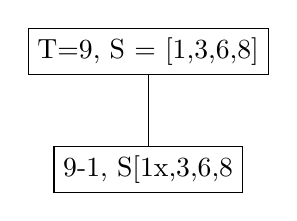
\begin{tikzpicture}[
      every node/.style = {minimum width = 4em, draw, rectangle},
      level/.style = {sibling distance = 50mm/#1}
      ]
      \node {T=9, S = [1,3,6,8]}
      child {node {9-1, S[1x,3,6,8}};
    \end{tikzpicture}
    \end{center}
    Do T = 8 != 0 nên ta tiếp tục sẽ lấy phần tử thứ 2, S[1] = 3 trừ tiếp cho T
    \begin{center}
    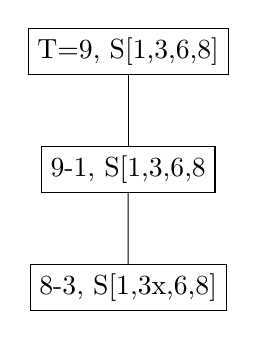
\begin{tikzpicture}[
      every node/.style = {minimum width = 4em, draw, rectangle},
      level/.style = {sibling distance = 50mm/#1}
      ]
      \node {T=9, S[1,3,6,8]}
      child {node {9-1, S[1,3,6,8}
            child {node{8-3, S[1,3x,6,8]}}};
    \end{tikzpicture}
    \end{center}
    Do T = 5 != 0 nên ta tiếp tục lấy phần tử thứ 3, s[2] = 6 trừ tiếp cho T
    \begin{center}
    \begin{tikzpicture}[
      every node/.style = {minimum width = em, draw, rectangle},
      level/.style = {sibling distance = 1cm/#1}
      ]
      \node {T=9, S[1,3,6,8]}
      child {node {9-1, S[1,3,6,8}
            child {node{8-3, S[1,3,6,8]}
                  child {node{5-6, S[1,3,6,8]}}}
            };
    \end{tikzpicture}
    \end{center}
    Do T < 0, Ta quay lui lại thay vì lấy phần tử thứ 3 trừ thì ta sẽ không trừ
    \begin{center}
    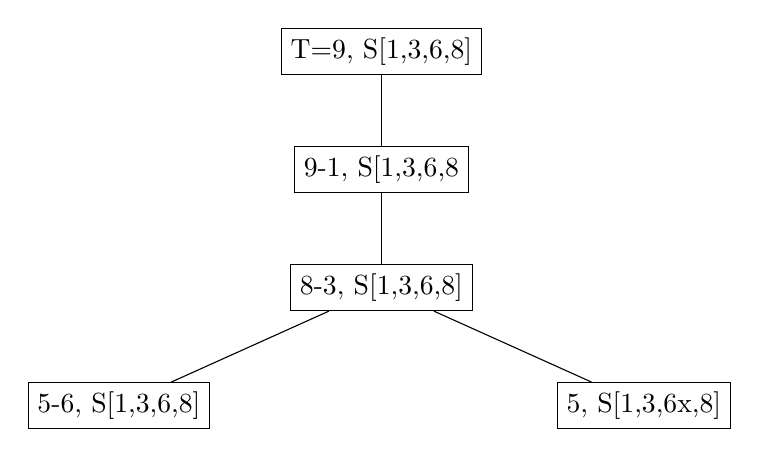
\begin{tikzpicture}[
      every node/.style = {minimum width = 4em, draw, rectangle},
      level/.style = {sibling distance = 20cm/#1}
      ]
      \node {T=9, S[1,3,6,8]}
      child {node {9-1, S[1,3,6,8}
            child {node{8-3, S[1,3,6,8]}
                  child {node{5-6, S[1,3,6,8]}}
                  child {node{5, S[1,3,6x,8]}}}
            };
    \end{tikzpicture}
    \end{center}
    
    
    Do T = 5 != 0, bên nhánh này thay vì ta lấy phần tử thứ 3 trừ thì ta lấy phần tử thứ 4 trừ cho 5, S[3] = 5
    \begin{center}
    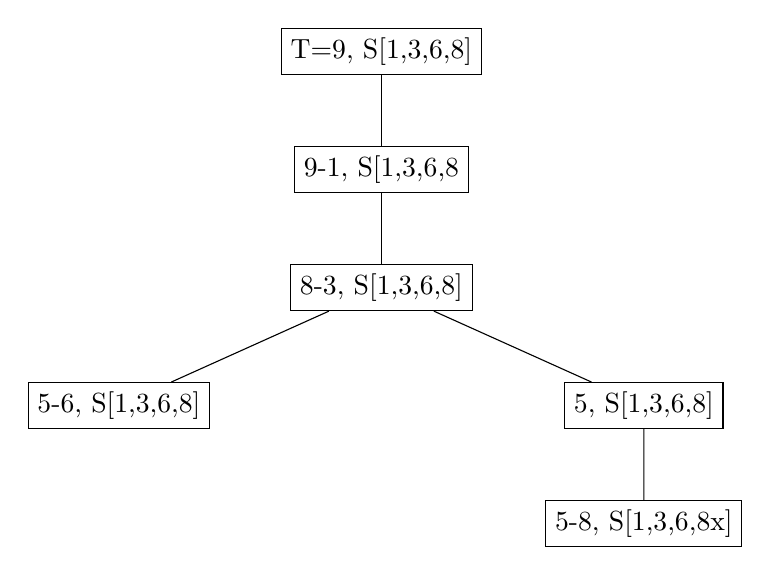
\begin{tikzpicture}[
      every node/.style = {minimum width = 4em, draw, rectangle},
      level/.style = {sibling distance = 20cm/#1}
      ]
      \node {T=9, S[1,3,6,8]}
      child {node {9-1, S[1,3,6,8}
            child {node{8-3, S[1,3,6,8]}
                  child {node{5-6, S[1,3,6,8]}}
                  child {node{5, S[1,3,6,8]}
                        child{node{5-8, S[1,3,6,8x]}}}}
            };
    \end{tikzpicture}
    \end{center}
    Do T < 0, nên ta sẽ loại nhánh này, quay lui và sang nhánh không trừ T cho phần tử thứ 4
    \begin{center}
    \hspace*{2cm}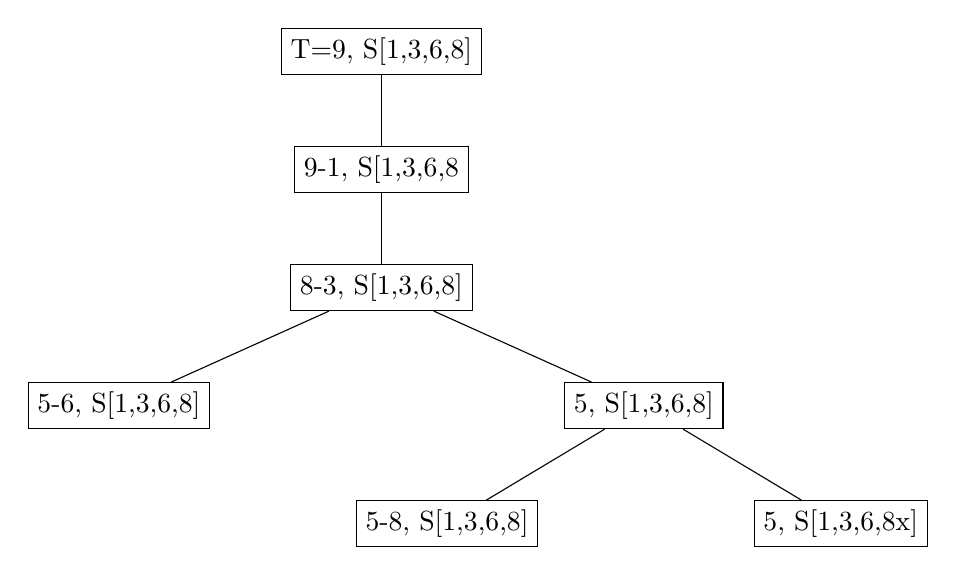
\begin{tikzpicture}[
      every node/.style = {minimum width = 4em, draw, rectangle},
      level/.style = {sibling distance = 20cm/#1}
      ]
      \node {T=9, S[1,3,6,8]}
      child {node {9-1, S[1,3,6,8}
            child {node{8-3, S[1,3,6,8]}
                  child {node{5-6, S[1,3,6,8]}}
                  child {node{5, S[1,3,6,8]}
                        child{node{5-8, S[1,3,6,8]}}
                        child{node{5, S[1,3,6,8x]}}}}
            };
    \end{tikzpicture}
    \end{center}
    
    
    Do nhánh này cũng sai ta sẽ quay lui lại đến trước khi trừ cho phần tử thứ 3, ta sẽ không lấy S[2] trừ cho T
    \begin{center}
    \hspace*{-2cm}\begin{tikzpicture}[
      every node/.style = {minimum width = 1em, draw, rectangle},parent node,
      level 1/.style={sibling distance=5cm},
    level 2/.style={sibling distance=11cm},
    level 3/.style={sibling distance=4cm},
    level 4/.style={sibling distance=5cm}]
      ]
      \node {T=9, S[1,3,6,8]}
      child {node {9-1, S[1,3,6,8}
            child {node{8-3, S[1,3,6,8]}
                  child {node{5-6, S[1,3,6,8]}}
                  child {node{5, S[1,3,6,8]}
                        child{node{5-8, S[1,3,6,8]}}
                        child{node{5, S[1,3,6,8]}}}}
            child{node{8,S[1,3x,6,8]}}
            };
    \end{tikzpicture}
    \end{center}
    \underline{Bước 2:} Tiếp tục lặp đề tìm toàn bộ các nhánh, nếu có nhánh nào mà T = 0, => có subset, hoặc nếu không thì không có Subset. Từ cây nhị phân này ta có thể truy ngược lại các phần tử có trong có trong subset
    \begin{center}
    \hspace*{-1.8cm}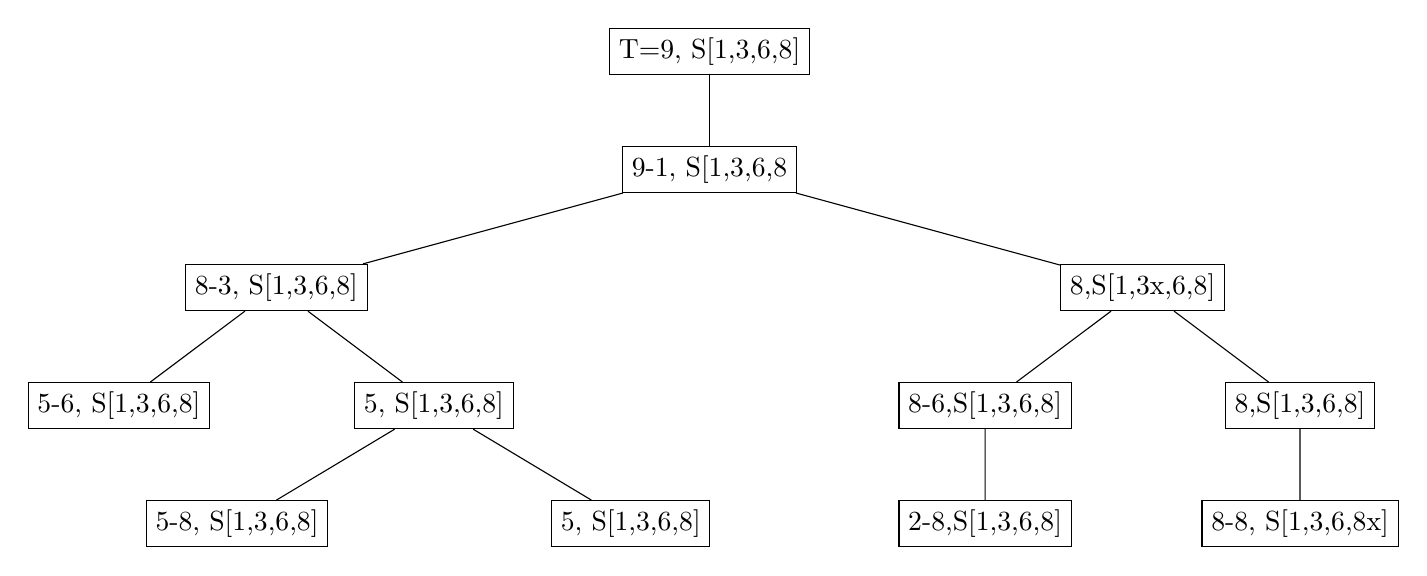
\begin{tikzpicture}[
      every node/.style = {minimum width = 1em, draw, rectangle},
      level 1/.style={sibling distance=5cm},
    level 2/.style={sibling distance=11cm},
    level 3/.style={sibling distance=4cm},
    level 4/.style={sibling distance=5cm}]
      ]
      \node {T=9, S[1,3,6,8]}
      child {node{9-1, S[1,3,6,8}
            child {node{8-3, S[1,3,6,8]}
                  child {node{5-6, S[1,3,6,8]}}
                  child {node{5, S[1,3,6,8]}
                        child{node{5-8, S[1,3,6,8]}}
                        child{node{5, S[1,3,6,8]}}}}
            child{node{8,S[1,3x,6,8]}
                  child{node{8-6,S[1,3,6,8]}
                  child{node{2-8,S[1,3,6,8]}}}
                    child{node{8,S[1,3,6,8]}
                    child{node{8-8, S[1,3,6,8x]}}}
                    }
            };
    \end{tikzpicture}
    \end{center}
    
    Trong ví dụ này thì ta thấy nhánh bên phải cùng có Subset = {1,8} cho ra Target = 9\\\\
    
    
    \underline{PseudoCode:}\\
    
    Subset Sum (S,i,T):\\
		\hspace*{1cm}If T == 0:\\
			\hspace*{2cm}Return true\\
		\hspace*{1cm}Else if T < 0 or i = 0:\\
			\hspace*{2cm}Return false\\
		\hspace*{1cm}Else:\\
		\hspace*{1cm}Return Subset Sum(S,i-1,T) or Subset Sum(S,i-1,T-X[i])\\
	
	\underline{Tham khảo:}\\ \url{https://www.youtube.com/watch?v=kyLxTdsT8ws&t=6s&ab_channel=AbdulBari}\\\\
	\url{https://courses.engr.illinois.edu/cs473/sp2017/notes/02-backtracking.pdf}
    \subsection{ \fontsize{16}{16}\selectfont\textbf{Phân tích độ phức tạp bằng toán}}
    \begin{center}
        \Tree[.N [.N-1 [.N-2 ]
               [.N-2 ]]
          [.N-1 [.N-2 ]
                [.N-2 [.N-3 ][.N-3 [.N-4 ][.N-4 ]]]]]\\
    \end{center}
    
    T(0) = 2 = c
    T(1) = 4 + c
    T(2) = 8 + c
    T(n) = 2*(T(n-1)) + C 
    => T(n) = 2*2*2* . . .* n lần => O({2^n})\\
    
    Space complexity: O({2^n})\\
    \newpage
    \subsection{ \fontsize{16}{16}\selectfont\textbf{Mã nguồn cài đặt}}
    
    \begin{lstlisting}[language=Python, caption=Code Demo]
	def subset_sum(array, target_sum, start=0, target_array=[]):  
    solutions = set()

    for idx in range(start, len(array)):
        target_array.append(array[idx])

        if sum(target_array) == target_sum:
            solutions.add(tuple(target_array))
            target_array.pop()
            solutions |= subset_sum(array, target_sum, start + 1)
            break

        solutions |= subset_sum(array, target_sum, idx + 1)
        target_array.pop()

    return solutions

a = list(map(int,input("\nEnter the numbers : ").strip().split()))
summ = int(input())

SS-BackTracking = subset_sum(a,summ)
print(SS-BackTracking)

\end{lstlisting}
Tham khảo: \url{https://stackoverflow.com/questions/56487300/recursive-backtracking-to-list-all-subsets-with-a-given-sum}\\
    \subsection{ \fontsize{16}{16}\selectfont\textbf{Cách thức phát sinh Input/Output để kiểm tra tính đúng đắn}}
    Cho một mảng S[1,2,...,n] với n $\in$ N* và Target Sum gọi là T $\in$ N*\\\\
    \textit{Base Case 1:} T = 0, $\forall$ S thì luôn có S' = $\varnothing$ cộng lại thành T, Output = True\\
    \hspace*{1.3cm}\textit{Case 2:} T < 0 hoặc S = $\varnothing$ thì Output = False\\\\
    \underline{Chứng minh:} Cho Len(S) = n > 1\\\\
    Dòng 7, \textit{Return Subset Sum (S,len(S)-1, T) or Subset Sum(S,len(S)-1,T-S[i])}: Theo như giải thích của phần Pseudo Code, Dòng này sẽ chạy hết toàn bộ các khả năng, và có 2 trường hợp sẽ xảy ra:\\\\
    \underline{Case 1:} Trừ từng phần tử trong S Cho T cho đến khi S = $\varnothing$, Nếu T = 0 tức là có Subset cộng được cho ra T\\\\
    \underline{Case 2 :} Nếu cho đến khi len(S) = 0 và T $\neq$ 0 thì không có subset nào.\\\\
    => Giải thuật đúng $\forall$ T $\in$ N* và S[1,2,...,n] với n $\in$ N* \\\\
    Tham khảo: \url{https://courses.engr.illinois.edu/cs473/sp2017/notes/02-backtracking.pdf}
    \newpage
    \subsection{ \fontsize{16}{16}\selectfont\textbf{Phân tích độ phức tạp bằng thực nghiệm}}
 n : kích thước mảng \\
T(n): thời gian chạy thực nghiệm tương ứng với kích thước mảng
    
    \begin{flushleft}
    
        \begin{adjustbox}{width=1.1\textwidth,center=\textwidth}
        *\begin{tabular}{|c|c|c|c|c|c|c|c|}
        \hline
        {n} & {T(n)} & {sqrt(n)*712.30043498} &{} & {lg(n)*1100.23489163} &{} &{n*78.99504265}&{}\\
     	\hline
        15&	0.062	&2758.727722&	7610236.567	&4298.497351&	18476546.47&	1184.92564&	1403901.845\\
        \hline
        16	&0.121	&2849.20174&	8117261.063	&4400.939567	&19367204.06&	1263.920682&	1597189.637\\
        \hline
        17&0.241&	2936.889931	&8623906.942	&4497.169236&	20222363.56	&1342.915725&	1802775.417 \\
        \hline
        18&	0.486&	3022.034807&	9129757.192&	4587.896982&	21044339.52	&1421.910768	&2020448.37\\
        \hline
        19	&0.963	&3104.845614	&9634087.278	&4673.718067	&21834639.92	&1500.90581	&2249828.434\\
        \hline
        20	&1.949&	3185.504386	&10135024.9	&4755.136089&	22592787.5&	1579.900853&	2489932.05\\
        \hline
        21&3.891	&3264.170661	&10629423.47	&4832.580884	&23316245.99	&1658.895896	&2739041.205\\
        \hline
        22	&7.864&	3340.985186	&11109696.84&	4906.422264	&23995873.06&	1737.890938	&2992993.207\\
        \hline
        23	&16.709&	3416.07288	&11555674.79	&4976.980699&	24604295.32	&1816.885981	&3240637.163\\
        \hline
        24&	38.536	&3489.545219&	11909464.63	&5044.53572	&25060033.2	&1895.881024&	3449730.537\\
        \hline
        25&	59.243&	3561.502175	&12265819.33	&5109.332612	&25503405.09	&1974.876066	&3669650.045\\
        \hline
        26	&127.159&	3632.033818&	12284147.49	&5171.587784&	25446261.76&	2053.871109&	3712219.551\\
        \hline
        27&260.217	&3701.221631	&11840512.87	&5231.493136	&24713586.42	&2132.866152	&3506814.845\\
        \hline
        28&	485.865&	3769.139619&	10779892.23&	5289.219622&	23072215.62&	2211.861194&	2979062.862\\
        \hline
        29	&1058.179	&3835.855235	&7715485.264	&5344.920194	&18376150.06	&2290.856237	&1519493.17\\
        \hline
        30	&2066.716&	3901.43016&	3366176.047&	5398.732243&	1110233224&	2369.85128&	91890.99768\\
        \hline
        {}&	{MSE}&{}&		9794160.43
&{}&		21795517.49
&{}&	2466600.583
\\
        \hline
        \end{tabular}
        \end{adjustbox}
    \end{flushleft}
    
    \begin{flushleft}
    
        \begin{adjustbox}{height=0.25\textwidth,width=1.1\textwidth,center=\textwidth}
        *\begin{tabular}{|c|c|c|c|c|c|c|c|}
        \hline
        {n*lg(n)*13.59733924} & {} & {n^2*1.8782545} &{} & {n^3*0.05704409} &{} &{(2^n)*1.92941792e-06}&{}\\
        \hline
        796.849752&	634870.7218&	422.6072625&	178544.4989&	192.5238038&	37041.5459&	6.32E-02&	1.49614E-06\\
        \hline
        870.2297114&	757089.1696	&480.833152	&231084.1731	&233.6525926	&54537.00476	&1.26E-01	&2.96625E-05\\
        \hline
        944.836521&	892260.6983&	542.8155505&	294387.1429&	280.2576142&	78409.30421	&2.53E-01&	0.000141435\\
        \hline
        1020.597927	&1040628.344	&608.554458	&369747.2496	&332.6811329&	110353.6063	&5.06E-01	&0.000391459\\
        \hline
        1097.449718	&1202283.122&	678.0498745	&458446.6356&	391.2654133&	152335.9738&	1.01E+00&	0.002359109\\
        \hline
        1175.33445	&1376833.413&	751.3018	&561529.6189	&456.35272&	206482.7407	&2.02E+00	&0.005496936\\
        \hline
        1254.200431	&1563273.673&	828.3102345&	679667.0742&	528.2853175&	274989.4002&	4.05E+00&	0.024112701\\
        \hline
        1334.0009	&1758639.077	&909.075178	&812181.5874	&607.4054703	&359449.9746	&8.09E+00	&0.052242096\\
        \hline
        1414.693349	&1954360.241&	993.5966305&	954309.4426&	694.055443&	458798.2039&	1.62E+01&	0.274439149\\
        \hline
        1496.238973	&2124897.956	&1081.874592	&1088555.418	&788.5775002	&562562.252	&3.24E+01	&38.01633497\\
        \hline
        1578.6022&	2308452.378&	1173.909063	&1242480.431&	891.3139063&	692341.993&	6.47E+01&	30.2227525\\
        \hline
        1661.750309&	2354970.486	&1269.700042	&1305400.033	&1002.606926	&766409.0709	&1.29E+02	&5.391892018\\
        \hline
        1745.653097	&2206520.399&	1369.247531	&1229948.718&	1122.798823&	744047.4022	&2.59E+02&	1.57480015\\
        \hline
        1830.2826&	1807458.684	&1472.551528	&973550.3045	&1252.231864	&587318.1697	&5.18E+02	&1027.790969\\
        \hline
        1915.612853&	735192.8118&	1579.612035&	271892.4095&	1391.248311&	110935.1659&	1.04E+03&	498.657557\\
        \hline
        2001.619681	&4237.530713	&1690.42905	&141591.8687	&1540.19043	&277229.1759	&2.07E+03	&24.80753864\\
        \hline


        \hline
        {}&	1420123.044
&{}&674582.2878
&{}&342077.5615
&{}&	101.6763161
\\
        \hline
        \end{tabular}
        \end{adjustbox}
    \end{flushleft}
    
    Vì MSE sai số toàn phương O({2^n})  = 101.6763161 bé nhất\\
    =>Theo kết quả thực nghiệm thì độ phức tạp của giải thuật này là O({2^n})



\newpage
\section{\fontsize{20}{20}\selectfont Design Algorithm: Dynamic Programing}

    \fontsize{16}{16}\selectfont
    \subsection{ \fontsize{16}{16}\selectfont\textbf{Phương pháp: Dynamic Programming}}
    Trong ngành khoa học máy tính, quy hoạch động (tiếng Anh: dynamic programming) là một phương pháp giảm thời gian chạy của các thuật toán thể hiện các tính chất của các bài toán con gối nhau (overlapping subproblem) và cấu trúc con tối ưu (optimal substructure).\\\\
    Nhà toán học Richard Bellman đã phát minh phương pháp quy hoạch động vào năm 1953. Ngành này đã được thành lập như là một chủ đề về kỹ nghệ và phân tích hệ thống đã được tổ chức IEEE thừa nhận.\\\\
    Tham khảo: \url{https://vi.wikipedia.org/wiki/Quy_ho%E1%BA%A1ch_%C4%91%E1%BB%99ng}
    \subsection{ \fontsize{16}{16}\selectfont\textbf{Pseudo code}}
    Input: Set[1,2,3,4,5,...,n] chứa n phần tử, mỗi phần tử là số nguyên dương\\
    \hspace*{2cm}Target sum = K là tổng mà ta cần tìm subset cho, giá trị Target sum là số nguyên dương
    
    \textit{Để giải quyết bài toàn này bằng phương pháp Dynamic programming thì ta làm như sau}:\\\\
    \hspace*{0.5cm}\underline{Bước 1:} ta tạo một ma trận 2 chiều type boolean gọi là M[i][j] với:\\
    \hspace*{1.8cm}-i : length của mảng chứa các phần tử cần có để tìm Subset\\
    \hspace*{1.8cm}-j : giá trị của target sum cần tìm subset\\\\
    
    \underline{Bước 2:} Nếu như phần tử ở vị trí thứ ith  trong Mảng  đang lớn hơn giá trị Sum lúc đấy ta copy đáp án của phần tử ở vị trí  M[i-1][j]. \\
    \hspace*{1.8cm}Nếu như phần tử ở vị trí thứ ith hiện tại đang nhỏ hơn thì ta so sánh phần tử ở vị trí M[i-1][j] và Phần tử ở vị trí M[i-1][j-Set[i]]\\
    
    \underline{Bước 3:} Lặp đến cuối ma trận, Nếu ô cuối là True thì tìm được Subset và ngược lại nếu là False thì Set không có Subset nào cộng lại ra được Target Sum\\
    
    \underline{Ví dụ:} Set là [1,2,3,4,5] và Target sum là 10\\
    
    Ta tạo ma trận với chiều dài là Target sum+1 và chiều rộng là len(Set)\\\\
    \begin{center}
        \begin{tabular}{|c|c|c|c|c|c|c|c|c|c|c|c|}
        \hline
        {}&{0}&{1}&{2}&{3}&{4}&{5}&{6}&{7}&{8}&{9}&{10}\\
        \hline
        1&&&&&&&&&&&\\
        \hline
        2&&&&&&&&&&&\\
        \hline
        4&&&&&&&&&&&\\
        \hline
        3&&&&&&&&&&&\\
        \hline
        5&&&&&&&&&&&\\
        \hline
         
    \end{tabular}
    \end{center}
    
    
    Cột 0 là giá trị target sum = 0, Do ta lúc nào cũng có thể tạo ta subset rỗng nên giá trị 0 luôn luôn đúng nên ta điền True vào toàn bộ cột 0\\
    \begin{center}
        \begin{tabular}{|c|c|c|c|c|c|c|c|c|c|c|c|}
        \hline
        {}&{0}&{1}&{2}&{3}&{4}&{5}&{6}&{7}&{8}&{9}&{10}\\
        \hline
        1&T&&&&&&&&&&\\
        \hline
        2&T&&&&&&&&&&\\
        \hline
        4&T&&&&&&&&&&\\
        \hline
        3&T&&&&&&&&&&\\
        \hline
        5&T&&&&&&&&&&\\
        \hline
    \end{tabular}
    \end{center}
    
    Tiếp theo là cột Target sum = 1, hàng 1 có giá trị 1 = Target sum nên là True do 1 = 1\\
    \begin{center}
        \begin{tabular}{|c|c|c|c|c|c|c|c|c|c|c|c|}
        \hline
        {}&{0}&{1}&{2}&{3}&{4}&{5}&{6}&{7}&{8}&{9}&{10}\\
        \hline
        1&T&T&&&&&&&&&\\
        \hline
        2&T&&&&&&&&&&\\
        \hline
        4&T&&&&&&&&&&\\
        \hline
        3&T&&&&&&&&&&\\
        \hline
        5&T&&&&&&&&&&\\
        \hline
    \end{tabular}
    \end{center}
    
    Cột tiếp theo Target sum = 2, kết quả là False do 1 != 2\\
    \begin{center}
        \begin{tabular}{|c|c|c|c|c|c|c|c|c|c|c|c|}
        \hline
        {}&{0}&{1}&{2}&{3}&{4}&{5}&{6}&{7}&{8}&{9}&{10}\\
        \hline
        1&T&T&F&&&&&&&&\\
        \hline
        2&T&&&&&&&&&&\\
        \hline
        4&T&&&&&&&&&&\\
        \hline
        3&T&&&&&&&&&&\\
        \hline
        5&T&&&&&&&&&&\\
        \hline
    \end{tabular}
    \end{center}
    
    Ta tiếp tục làm vậy đến cột target sum = 10\\
    \begin{center}
        \begin{tabular}{|c|c|c|c|c|c|c|c|c|c|c|c|}
        \hline
        {}&{0}&{1}&{2}&{3}&{4}&{5}&{6}&{7}&{8}&{9}&{10}\\
        \hline
        1&T&T&F&F&F&F&F&F&F&F&F\\
        \hline
        2&T&&&&&&&&&&\\
        \hline
        4&T&&&&&&&&&&\\
        \hline
        3&T&&&&&&&&&&\\
        \hline
        5&T&&&&&&&&&&\\
        \hline
    \end{tabular}
    \end{center}
    
    Đến hàng 2 có giá trị = 2, ở cột target sum = 1 do 1<2 nên ta copy giá trị ở hàng 1\\
    \begin{center}
        \begin{tabular}{|c|c|c|c|c|c|c|c|c|c|c|c|}
        \hline
        {}&{0}&{1}&{2}&{3}&{4}&{5}&{6}&{7}&{8}&{9}&{10}\\
        \hline
        1&T&T&F&F&F&F&F&F&F&F&F\\
        \hline
        2&T&T&&&&&&&&&\\
        \hline
        4&T&&&&&&&&&&\\
        \hline
        3&T&&&&&&&&&&\\
        \hline
        5&T&&&&&&&&&&\\
        \hline
    \end{tabular}
    \end{center}
    
    Đến cột target sum = 2 cũng giống như ở hàng 1 do 2=2 nên cột này là T\\
    \begin{center}
        \begin{tabular}{|c|c|c|c|c|c|c|c|c|c|c|c|}
        \hline
        {}&{0}&{1}&{2}&{3}&{4}&{5}&{6}&{7}&{8}&{9}&{10}\\
        \hline
        1&T&T&F&F&F&F&F&F&F&F&F\\
        \hline
        2&T&T&T&&&&&&&&\\
        \hline
        4&T&&&&&&&&&&\\
        \hline
        3&T&&&&&&&&&&\\
        \hline
        5&T&&&&&&&&&&\\
        \hline
    \end{tabular}
    \end{center}
    
    Đến cột Target Sum = 3, do 3 >2 nên ta nhìn vào hàng trước đó là hàng 1, lấy Target sum - giá trị ở hàng thứ ith là 3 -2 =1\\
    Ta thấy cột Target Sum = 1 ở hàng 1 là T, ngoài ra ta cũng phải xem ở vị trí target sum = 3 hiện tại ở hàng 1 là giá trị gì, lần này là F.\\
    Ta sẽ lấy cột nào có giá trị T làm giá trị cho vị trí hiện tại, nếu cả 2 đều là False thì giá trị ở vị trí hiện tại sẽ là False\\
    \begin{center}
        \begin{tabular}{|c|c|c|c|c|c|c|c|c|c|c|c|}
        \hline
        {}&{0}&{3-2}&{2}&{3}&{4}&{5}&{6}&{7}&{8}&{9}&{10}\\
        \hline
        1&T&T<-&F&F&F&F&F&F&F&F&F\\
        \hline
        2&T&T&T&T&&&&&&&\\
        \hline
        4&T&&&&&&&&&&\\
        \hline
        3&T&&&&&&&&&&\\
        \hline
        5&T&&&&&&&&&&\\
        \hline
    \end{tabular}
    \end{center}
    
    Tương tự như trên là cột Target sum = 4, ta nhìn vào hàng trước đó là hàng 1, lùi 2 bước 4-2 = 2, giá trị ở đây là F nên giá trị ở hàng 2 cột 4 cũng là False\\
    \begin{center}
        \begin{tabular}{|c|c|c|c|c|c|c|c|c|c|c|c|}
        \hline
        {}&{0}&{1}&{4-2}&{3}&{4}&{5}&{6}&{7}&{8}&{9}&{10}\\
        \hline
        1&T&T&F<-&F&F&F&F&F&F&F&F\\
        \hline
        2&T&T&T&T&F&&&&&&\\
        \hline
        4&T&&&&&&&&&&\\
        \hline
        3&T&&&&&&&&&&\\
        \hline
        5&T&&&&&&&&&&\\
        \hline
    \end{tabular}
    \end{center}
    
     Tương tự như trên là cột Target sum = 4, ta nhìn vào hàng trước đó là hàng 1, lùi 2 bước 4-2 = 2, giá trị ở đây là F nên giá trị ở hàng 2 cột 4 cũng là False\\
    \begin{center}
        \begin{tabular}{|c|c|c|c|c|c|c|c|c|c|c|c|}
        \hline
        {}&{0}&{1}&{4-2}&{3}&{4}&{5}&{6}&{7}&{8}&{9}&{10}\\
        \hline
        1&T&T&F<-&F&F&F&F&F&F&F&F\\
        \hline
        2&T&T&T&T&F&&&&&&\\
        \hline
        4&T&&&&&&&&&&\\
        \hline
        3&T&&&&&&&&&&\\
        \hline
        5&T&&&&&&&&&&\\
        \hline
    \end{tabular}
    \end{center}
    
    Lặp lại cho đến hết hàng 3 có giá trị là 4\\
    \begin{center}
        \begin{tabular}{|c|c|c|c|c|c|c|c|c|c|c|c|}
        \hline
        {}&{0}&{1}&{2}&{3}&{4}&{5}&{6}&{7}&{8}&{9}&{10}\\
        \hline
        1&T&T&F&F&F&F&F&F&F&F&F\\
        \hline
        2&T&T&T&T&F&F&F&F&F&F&F\\
        \hline
        4&T&T&T&T&T&T&T&F&F&F&F\\
        \hline
        3&T&&&&&&&&&&\\
        \hline
        5&T&&&&&&&&&&\\
        \hline
    \end{tabular}
    \end{center}
    Ở hàng 4 giá trị là 3, cột Target sum = 7, như đã nói ở trên ta xem vị trí target sum = 7 ở hàng trước là giá trị gì, trong trường hợp này là False, và vị trí target sum - giá trị hàng hiện tại lúc này là = 3, vị trí 7-3 = 4, trong trường hợp này là T, ta lấy giá trị T\\
    \begin{center}
        \begin{tabular}{|c|c|c|c|c|c|c|c|c|c|c|c|}
        \hline
        {}&{0}&{1}&{2}&{3}&{4}&{5}&{6}&{7}&{8}&{9}&{10}\\
        \hline
        1&T&T&F&F&F&F&F&F&F&F&F\\
        \hline
        2&T&T&T&T&F&F&F&F&F&F&F\\
        \hline
        4&T&T&T&T&T&T&T&F&F&F&F\\
        \hline
        3&T&T&T&T&T&T&T&T&&&\\
        \hline
        5&T&&&&&&&&&&\\
        \hline
    \end{tabular}
    \end{center}
    
    Tiếp tục lặp cho đến cuối Matrix\\
    \begin{center}
        \begin{tabular}{|c|c|c|c|c|c|c|c|c|c|c|c|}
        \hline
        {}&{0}&{1}&{2}&{3}&{4}&{5}&{6}&{7}&{8}&{9}&{10}\\
        \hline
        1&T&T&F&F&F&F&F&F&F&F&F\\
        \hline
        2&T&T&T&T&F&F&F&F&F&F&F\\
        \hline
        4&T&T&T&T&T&T&T&F&F&F&F\\
        \hline
        3&T&T&T&T&T&T&T&T&T&T&F\\
        \hline
        5&T&T&T&T&T&T&T&T&T&T&T\\
        \hline
    \end{tabular}
    \end{center}
    
    Kết luận ở cột 10 hàng 5 là T => Có subset cộng lại = target sum = 10\\\\
    Ta cũng có thể dò lại bảng và biết được các giá trị nào cộng lại ra Target Sum
    \\
    \\
    \underline{Pseudo code:} Mã giả áp dụng ý tưởng trên:\\\\
    Subset-sum(Set,Target Sum):\\
	\hspace*{0.8cm}Initialize M[i][0] = False, i = 0, . . . n\\
	\hspace*{0.8cm}Initialize M[0][j] =False, j = 1, . . . Sum+1\\
	\hspace*{0.8cm}for i from 0,...,n\\
	\hspace*{0.8cm}\hspace*{0.8cm} M[i][0] <- True\\
	\hspace*{0.8cm}For i from 1, . . ., n:\\
		\hspace*{0.8cm}\hspace{0.8cm}For j from 1, . . ., Sum:\\
			\hspace*{0.8cm}\hspace{0.8cm}\hspace{0.8cm}If j < X[i-1]:\\
				\hspace*{0.8cm}\hspace{0.8cm}\hspace{0.8cm}\hspace{0.8cm}M[i][j] <- M[i-1][j]\\
			\hspace*{0.8cm}\hspace{0.8cm}\hspace{0.8cm}If j >= X[i-1]:\\
				\hspace*{0.8cm}\hspace{0.8cm}\hspace{0.8cm}\hspace{0.8cm}M [i][j] <- M[i-1][j] or 
    M [i - 1][j-X [i-1]]\\\\
	\hspace*{0.8cm}Return M[len(set)-1][Sum]\\\\
	
	\underline{Tham khảo:} \url{https://www.youtube.com/watch?v=s6FhG--P7z0&t=327s&ab_channel=TusharRoy-CodingMadeSimple}\\\\
	\url{https://www.geeksforgeeks.org/subset-sum-problem-dp-25/}\\\\
    \subsection{ \fontsize{16}{16}\selectfont\textbf{Phân tích độ phức tạp bằng phương pháp toán học}}
    Do Matrix[i][j] được tạo ra từ Len(set) và Sum nên độ phức tạp\\
    Time  Complexity là O(len(set)*sum)\\
    Space Complexity là O(len(set)*sum)\\\\
    \underline{Tham khảo:} \\
    \url{https://www.geeksforgeeks.org/subset-sum-problem-dp-25/}\\
    \url{https://www.faceprep.in/data-structures/space-complexity/}\\\\
    
    \newpage
    \subsection{ \fontsize{16}{16}\selectfont\textbf{Mã nguồn cài đặt}}
    \begin{lstlisting}[language=Python, caption=Code Demo]
	
def find_subset(weight: list, req_sum: int):
    l = len(weight)

    # ROWS : array
    # COL : range(sum)
    row = l
    col = req_sum + 1

    # 2d array storing Sum
    dp_array = [[0] * col for i in range(row)]

    for i in range(row):
        for j in range(1, col):
            # Row 0
            if i == 0:
                if j >= weight[i]:
                    dp_array[i][j] = weight[i]
                else:
                    continue
            else:
                if j - weight[i] >= 0:
                    dp_array[i][j] = max(dp_array[i - 1][j], (weight[i] + dp_array[i - 1][j - weight[i]]))
                elif j >= weight[i]:
                    # take from row above it
                    dp_array[i][j] = max(dp_array[i - 1][j], weight[i])
                else:
                    dp_array[i][j] = dp_array[i - 1][j]

    # Find out which Numbers should be in the subset
    # give from index 0
    row -= 1
    col -= 1
    sum_subset = []

    # check if the Subset is possible : if not, return None
    if dp_array[row][col] != req_sum:
        return None

    # get the subset
    while col >= 0 and row >= 0 and req_sum > 0:
        # First Row
        if (row == 0):
            sum_subset.append(weight[row])
            break

        # Bottom-Right most ele
        if (dp_array[row][col] != dp_array[row - 1][col]):
            # print(req_sum,' : ',dp_array[row][col],dp_array[row-1][col],' : ',weight[row])
            sum_subset.append(weight[row])
            req_sum -= weight[row]
            col -= weight[row]
            row -= 1
        else:
            row -= 1

    return sum_subset

# main
if __name__ == "__main__":
    array = list(map(int, input().split()))
    req_sum = int(input())

    # Sort by ascending order
    array.sort()
    sum_subset = find_subset(array, req_sum)

    # If Sum is not possible
    if sum_subset is None:
        print("Sum :", req_sum, "is not possible")
    else:
        print("Subset for sum", req_sum, ' :')
        print(' '.join(str(x) for x in sum_subset))
    
\end{lstlisting}
    Tham khảo: \url{https://github.com/kaushikthedeveloper/GeeksforGeeks-python/blob/master/Scripts/Subset%20sum%20problem.py}
\\
    \subsection{ \fontsize{16}{16}\selectfont\textbf{Cách thức phát sinh Input/Output để kiểm tra tính đúng đắn}}
    Ví dụ: List S[1,3,4,5] và Target T = 7\\
    => Matrix[i][j] với i = len(S) và j = T
    \begin{center}
        \begin{tabular}{|c|c|c|c|c|c|c|c|c|}
        \hline
        {}&{0}&{1}&{2}&{3}&{4}&{5}&{6}&{7}\\
        \hline
        1&T&&&&&&&\\
        \hline
        3&T&&&&&&&\\
        \hline
        4&T&&&&&&&\\
        \hline
        5&T&&&&&&&\\
        \hline
    \end{tabular}
    \end{center}
    
    Ta giả sử rằng có thêm 1 hàng nữa là hàng rỗng 0 trước 1
    \begin{center}
        \begin{tabular}{|c|c|c|c|c|c|c|c|c|}
        \hline
        {}&{0}&{1}&{2}&{3}&{4}&{5}&{6}&{7}\\
        \hline
        0&T&F&F&F&F&F&F&F\\
        \hline
        1&T&&&&&&&\\
        \hline
        3&T&&&&&&&\\
        \hline
        4&T&&&&&&&\\
        \hline
        5&T&&&&&&&\\
        \hline
    \end{tabular}
    \end{center}
    Do hàng rỗng này chỉ cho kết quả cho Target = 0 nên toàn bộ cột Target khác = 0\\\\
    Tiếp tục theo thuật toán ở phần 2: Pseudo code thì nếu 
    j >= S[i-1], lúc này S[i-1] = 1 thì ta so sánh 2 kết quả ở M[i-1][j] và M[i-1][j-S[i-1]]. Có nghĩa là ta lấy kết quả của M[i-1][j] hoặc M[i-1][j-S[i-1]] cộng với S[i-1] = j thì đúng\\\\
    Hiện tại M[i-1][j] = 1 và M[i-1][j-S[i-1]] = 0\\
    S[i-1] + M[i-1][j] = 2 và S[i-1] + M[i-1][j-S[i-1]] = 1 == j => Kết quả là đúng
    \begin{center}
        \begin{tabular}{|c|c|c|c|c|c|c|c|c|}
        \hline
        {}&{0}&{1}&{2}&{3}&{4}&{5}&{6}&{7}\\
        \hline
        0&T&F&F&F&F&F&F&F\\
        \hline
        1&T&T&&&&&&\\
        \hline
        3&T&&&&&&&\\
        \hline
        4&T&&&&&&&\\
        \hline
        5&T&&&&&&&\\
        \hline
    \end{tabular}
    \end{center}
    Tiếp tục với j = 2, điều kiện vẫn là j >= S[n-1] = 1 ta tiếp tục\\
    M[i-1][j] = 2 và  M[i-1][j-S[i-1]] = 1\\
     S[i-1] + M[i-1][j] = 3 và S[i-1] + M[i-1][j-S[i-1]] = 2 => kết quả là F.
     \begin{center}
        \begin{tabular}{|c|c|c|c|c|c|c|c|c|}
        \hline
        {}&{0}&{1}&{2}&{3}&{4}&{5}&{6}&{7}\\
        \hline
        0&T&F&F&F&F&F&F&F\\
        \hline
        1&T&T&F&&&&&\\
        \hline
        3&T&&&&&&&\\
        \hline
        4&T&&&&&&&\\
        \hline
        5&T&&&&&&&\\
        \hline
    \end{tabular}
    \end{center}
    Ta tiếp tục làm cho đến hết hàng \\
    \begin{center}
        \begin{tabular}{|c|c|c|c|c|c|c|c|c|}
        \hline
        {}&{0}&{1}&{2}&{3}&{4}&{5}&{6}&{7}\\
        \hline
        0&T&F&F&F&F&F&F&F\\
        \hline
        1&T&T&F&F&F&F&F&F\\
        \hline
        3&T&&&&&&&\\
        \hline
        4&T&&&&&&&\\
        \hline
        5&T&&&&&&&\\
        \hline
    \end{tabular}
    \end{center}
    Tại j = 1, S[i-1] = 3 do J < S[i-1] nên ta chỉ đơn giản là hạ kết quả từ M[i-1][j] xuống làm kết quả.\\
    \begin{center}
        \begin{tabular}{|c|c|c|c|c|c|c|c|c|}
        \hline
        {}&{0}&{1}&{2}&{3}&{4}&{5}&{6}&{7}\\
        \hline
        0&T&F&F&F&F&F&F&F\\
        \hline
        1&T&T&F&F&F&F&F&F\\
        \hline
        3&T&T&&&&&&\\
        \hline
        4&T&&&&&&&\\
        \hline
        5&T&&&&&&&\\
        \hline
    \end{tabular}
    \end{center}
    Tiếp tục lặp như vậy cho đến hết bảng\\
    \begin{center}
        \begin{tabular}{|c|c|c|c|c|c|c|c|c|}
        \hline
        {}&{0}&{1}&{2}&{3}&{4}&{5}&{6}&{7}\\
        \hline
        0&T&F&F&F&F&F&F&F\\
        \hline
        1&T&T&F&F&F&F&F&F\\
        \hline
        3&T&T&F&T&T&F&F&F\\
        \hline
        4&T&T&F&T&T&T&F&T\\
        \hline
        5&T&T&F&T&T&T&T&T\\
        \hline
    \end{tabular}
    \end{center}
    Do giải thuật này tìm tổng của toàn bộ các subset có trong S và đưa kết quả vào trong bảng, Nếu như có subset mà tìm ra được Target thì kết quả ở ô dưới cùng phải sẽ là True và ngược lại => Giải thuật đúng\\\\
    Tham khảo: \url{https://www.youtube.com/watch?v=s6FhG--P7z0&t=327s&ab_channel=TusharRoy-CodingMadeSimple}
    
    \subsection{ \fontsize{16}{16}\selectfont\textbf{Phân tích độ phức tạp bằng thực nghiệm}}
    
  n : kích thước mảng \\
 Sum: tổng mà các subset cần đạt được\\
T(n): thời gian chạy thực nghiệm tương ứng với kích thước mảng\\
T(Sum): thời gian chạy thực nghiệm tương ứng với độ lớn của tổng\\\\

\textit{Bởi độ phức tạp cần chứng minh là O(n*Sum)=> n và Sum tỉ lệ thuận\\
Nên n tăng O(n*Sum) tăng, n giảm O(n*Sum) giảm\\
Tương tự, Sum tăng O(n*Sum) tăng, Sum giảm O(N*Sum) giảm}
    \begin{itemize}
    \item     Thay đổi n , Sum cố định
    \end{itemize}
    \begin{flushleft}
        \begin{adjustbox}{width=1.1\textwidth,center=\textwidth}
        *\begin{tabular}{|c|c|c|c|c|c|c|c|}
        \hline
        {n} & {T(n)} & {sqrt(n)*1.63250947} &{} & {lg(n)*7.05058841} &{} &{n*0.04568461}&{}\\
        \hline
        10 &	0.447&	5.162448227&	22.23545198&	23.42154772&	527.8298432&	0.4568461&	9.69457E-05\\
        \hline
        20	&0.857&	7.300804298&	41.52261383&	30.47213613&	877.0562883&	0.9136922&	0.003214006\\
        \hline
        50	&2.128	&11.54358517	&88.65324402	&39.79250704	&1418.615091	&2.2842305	&0.024407969\\
        \hline
        80	&3.434&	14.6016086&	1247154817&	44.57331295&	1692.44307&	3.6547688&	0.048738863\\
        \hline
        100	&4.247	&16.3250947	&145.8803716	&46.84309545	&1814.427348	&4.568461	&0.103337175\\
        \hline
        150	&7.271&	19.99407601&	161.8766631&	50.96742528&	1909.377582&	6.8526915&	0.174982001\\
        \hline
        200	&8.42&	23.08717033&	215.1258855&	53.89368386&	2067.855924&	9.136922&	0.513977154\\
        \hline
        250	&10.787	&25.81224113	&225.7578712	&56.16346635	&2059.023699	&11.4211525	&0.402149393\\
        \hline
        300	&14.421&	28.27589346&	191.9580728&	58.01801369&	1900.699602&	13.705383&	0.512107691\\
        \hline
        350	&15.137&	30.54145559&	237.2972519&	59.58601112&	1975.714589&	15.9896135&	0.72694978\\
        \hline
        400	&17.415	&32.6501894	&232.1109961	&60.94427227	&1894.797544	&18.273844	&0.737613016\\
        \hline
        450	&19.875&	34.6307555&	217.7323203&	62.14234352&	1786.528328&	20.5580745&	0.466590773\\
        \hline
        500	&22.077	&36.50402149	&208.138949	&63.21405476	&1692.257275	&22.842305	&0.585691743\\
        \hline
        550	&24.537	&38.28574073&	189.0278717&	64.18353551&	1571.847778&	25.1265355&	0.347552106\\
        \hline
        600	&26.962	&39.98815202	&169.6806364	&65.0686021	&1452.113123	&27.410766	&0.201390923\\
        \hline
        650	&29.019&	41.62098822&	158.8101071&	65.88278443&	1358.938602&	29.6949965&	0.456971268\\
        \hline
        700	&31.566	&43.19214071	&135.1671477	&66.63659953	&1229.946951	&31.979227	&0.170756554\\
        \hline
        750	&33.724&	44.7081131&	120.6507407&	67.33838459&	1129.926851&	34.2634575&	0.291014394\\
        \hline
        800	&36.592	&46.17434066	&91.82125259	&67.99486068&	986.1396588	&36.547688	&0.001963553\\
        \hline
        850	&38.624	&47.59542094&	80.48639363&	68.61152517&	899.2516661&	38.8319185&	0.043230103\\
        \hline
        900	&40.843	&48.9752841	&66.13404468&	69.19293193&	803.7186402&	41.116149&	0.074610376\\
        \hline
        950	&43.157&	50.31732118&	51.27019946&	69.74289553&	706.8098412&	43.4003795&	0.059233581\\
        \hline
        1000	&46.252	&51.62448227	&28.86356574	&70.26464317	&576.6070322	&45.68461	&0.321931412\\

        \hline
        {}&	{MSE}&{}&		139.3442232
&{}&		1405.735927
&{}&	0.272543947\\
        \hline
        \end{tabular}
        \end{adjustbox}
    \end{flushleft}
    
    \begin{flushleft}
    
        \begin{adjustbox}{width=1.1\textwidth,center=\textwidth}
        *\begin{tabular}{|c|c|c|c|c|c|c|c|}
        \hline
        {n*lg(n)*0.00451603} & {} & {n^2*4.43992465e-05} &{} & {n^3*4.70042114e-08} &{} \\
        \hline
        0.150019269 &0.088197554	&0.004439925	&0.19585942	    &4.70042E-05&	0.19976698\\
        \hline
        0.390359139	&0.217753693	&0.017759699	&0.704324283	&0.000376034&	0.73380462\\\hline
        1.274391193	&0.728647995	&0.110998116	&4.068296599	&0.005875526&	4.503412281\\\hline
        2.284001355	&1.322496884	&0.284155178	&9.921522405	&0.024066156&	11.62764882\\\hline
        3.000385387	&1.554047994	&0.443992465	&14.46286631	&0.047004211&	17.63996462\\\hline
        4.896834311	&5.636662721	&0.998983046	&39.33819667	&0.158639213&	50.58567596\\\hline
        6.903976774	&2.298326423	&1.77596986	    &44.1431365	    &0.376033691&	64.70539398\\\hline
        8.993430201	&3.216892625	&2.774952906	&64.19289863	&0.734440803&	101.0539464\\\hline
        11.14847762	&10.70940272	&3.995932185	&108.6820389	&1.269113708&	172.972113\\\hline
        13.35807302	&3.164581196	&5.438907696	&94.05299433	&2.015305564&	172.1788649\\\hline
        15.61436555	&3.242284432	&7.10387944	    &106.3192072	&3.00826953	&207.5538828\\\hline
        17.91148512	&3.855390673	&8.990847416	&118.4647775	&4.283258764&	243.1023948\\\hline
        20.2448754	&3.356680544	&11.09981163	&120.4986646	&5.875526425&	262.487746\\\hline
        22.61089646	&3.709874836	&13.43077207	&123.3482989	&7.820325672&	279.4472006\\\hline
        25.00657324	&3.823693804	&15.98372874	&120.5224399	&10.15290966&	282.545518\\\hline
        27.42942842	&2.526737802	&18.75868165	&105.2741327	&12.90853156&	259.5471935\\\hline
        29.87736704	&2.851481266	&21.75563079	&96.24334413	&16.12244451&	238.5034062\\\hline
        32.34859425	&1.891740966	&24.97457616	&76.5524176	    &19.82990168&	193.045968\\\hline
        34.84155509	&3.064057366	&28.41551776	&66.85486182	&24.06615624&	156.896762\\\hline
        37.35488938	&1.610641763	&32.0784556	    &42.84415154	&28.86646133&	95.20956097\\\hline
        39.88739725	&0.913176624	&35.96338967	&23.81059702	&34.26607011&	43.25600677\\\hline
        42.43801236	&0.516943227	&40.07031997	&9.527593631	&40.30023575&	8.161101985\\\hline
        45.0057808	&1.553062287	&44.3992465	    &3.432695532	&47.0042114	&0.56582199\\

        \hline
        {}&	2.689251104
&{}&60.58501375
&{}&124.6314415
\\
        \hline
        \end{tabular}
        \end{adjustbox}
    \end{flushleft}
    
    Vì MSE sai số toàn phương O(n) = 0.272543947 bé nhất\\
    =>Theo kết quả thực nghiệm thì độ phức tạp giải thuật là  O(n) nếu Sum cố định và n thay đổi
    
    \begin{itemize}
    \item     Thay đổi Sum, n cố định
    \end{itemize}
    
    \begin{flushleft}
        \begin{adjustbox}{width=1.1\textwidth,center=\textwidth}
        *\begin{tabular}{|c|c|c|c|c|c|c|c|}
        \hline
        {Sum} & {T(Sum)} & {sqrt(Sum)*0.06922314} &{} & {lg(Sum)*7.80286957} &{} &{Sum*5.35591186e-05}&{}\\
        \hline
        1000	&0.024&	2.189027892&4.687345773&	77.76171494&	6043.152323&	0.053559119&	0.000873741\\\hline
        5000&	0.141&	4.894815171&22.59875868	&95.87941701&	9165.844492	&0.267795593	&0.016077122\\\hline
        10000&	0.374&	6.922314&   42.88041624	&103.6822866&	10672.60208	&0.535591186	&0.026111711\\\hline
        20000&	0.892&	9.789630342&79.1678257	&111.4851562&	12230.84619&	1.071182372	&0.032106322\\\hline
        30000&	1.398&	11.98979955&	112.1862178&116.0495422&	13144.97614&	1.606773558&	0.043586399\\\hline
        40000&	1.956&	13.844628	&141.3394757&	119.2880257	&13766.80426&	2.142364744	&0.034731818\\\hline
        50000&	2.448&	15.47876467	&169.8008278&	121.7999887&	14244.8972&	2.67795593	&0.05287973\\\hline
        60000&	2.95&	16.95613714	&196.1718776&	123.8524118&	14617.39318&	3.213547116&	0.069457082\\\hline
        70000&	3.454&	18.31472134	&220.8410388&	125.5877109&	14916.64333&	3.749138302	&0.087106617\\\hline
        80000&	3.976&	19.57926068	&243.461744	&127.0908953&	15157.27744	&4.284729488	&0.095313897\\\hline
        90000&	4.585&	20.766942	&261.8552469&	128.4167979&	15334.31417&	4.820320674&	0.05537582\\\hline
        100000&	5.248&	21.89027892	&276.9654476&	129.6028582	&15464.13076&	5.35591186	&0.01164497\\\hline
        200000&	10.252&	30.95752933&	428.7189449&137.4057278	&16168.07049&	10.71182372	&0.211437853\\\hline
        300000&	15.53&	37.91507528&	501.0915953&141.9701139	&15987.1024	&16.06773558	&0.289159554\\\hline
        400000&	20.658&	43.78055784	&534.652681	&145.2085974&	15512.8513	&21.42364744	&0.586216002\\\hline
        500000&	25.684&	48.94815171&	541.2207547&147.7205603&	14892.92205&	26.7795593	&1.20025018\\\hline
        600000&	31.035&	53.62001368&	510.0828429&149.7729835	&14098.70872&	32.13547116	&1.211036774\\\hline
        700000&	36.129&	57.91623415&	474.6835719&151.5082825	&13312.37883&	37.49138302	&1.856087493\\\hline
        800000&	41.845&	61.91505866&	402.8072547&153.0114669	&12357.98337&	42.84729488	&1.004595026\\\hline
        900000&	47.575&	65.67083676&	327.4593079&154.3373696	&11398.20355&	48.20320674	&0.394643708\\\hline
        1000000&52.331&	69.22314&	285.3443938	&155.5234299	&10648.67758&	53.5591186	&1.508275296\\\hline
        1500000	&79.643&84.7806857&	26.39581432	&160.087816 	&6471.368416&	80.3386779	&0.483967741\\\hline
        2000000	&108.299&97.89630342&108.2160962&	163.3262994	&3028.003684&	107.1182372&	1.39420079\\

        \hline
        {}&	{MSE}&{}&		263.836972&{}&		12982.1431&{}&	0.42140613
\\
        \hline
        \end{tabular}
        \end{adjustbox}
    \end{flushleft}
    
    \begin{flushleft}
    
        \begin{adjustbox}{width=1.1\textwidth,center=\textwidth}
        *\begin{tabular}{|c|c|c|c|c|c|c|c|}
        \hline
        {Sum*lg(Sum)*0.00451603} & {} & {Sum^2*4.43992465e-05} &{} & {Sum^3*4.70042114e-08} &{} \\
        \hline
        0.025796706&	3.22815E-06&	2.88463E-05&0.000574616&	1.40001E-08&	0.000575999\\\hline
        0.159035405	&0.000325276	&0.000721156&	0.019678154&	1.75001E-06&	0.019880507\\\hline
        0.343956085&	0.000902637	&0.002884626&	0.137726621&	1.40001E-05&	0.139865528\\\hline
        0.73968272&	0.023200554	&0.011538502&   	0.775212449&	0.000112001&	0.795464203\\\hline
        1.154949824&	0.059073388&	0.02596163&	1.882489287&	0.000378002&	1.953347249\\\hline
        1.582906538&	0.139198731	&0.04615401	&   3.647511706&	0.000896005&	3.82243163\\\hline
        2.020299158	&0.18292801	&0.07211564&    	5.644826491&	0.00175001&	5.984139012\\\hline
        2.465211297	&0.235020087&	0.103846522&	8.100589621&	0.003024018&	8.68466744\\\hline
        2.916376669	&0.289038846&	0.141346655&	10.97367218&	0.004802028&	11.89696665\\\hline
        3.372895273	&0.363735311&	0.184616039&	14.37459234&	0.007168042&	15.75162711\\\hline
        3.834094181	&0.563859549&	0.233654674&	18.93420614&	0.01020606&	20.92873959\\\hline
        4.299451063	&0.899745085&	0.288462561&	24.59701161&	0.014000082&	27.39475514\\\hline
        9.116607621	&1.289115854&	1.153850244&	82.77632898&	0.112000659&	102.8195866\\\hline
        14.12916888	&1.962327821&	2.596163049&	167.2841383&	0.378002225&	229.5830366\\\hline
        19.26862623	&1.930359473&	4.615400976&	257.3649834&	0.896005274&	390.5364356\\\hline
        24.50244265	&1.396077781&	7.211564025&	341.2308909&	1.7500103&	572.835863\\\hline
        29.81145425	&1.497064212&	10.3846522&	    426.4368644&	3.024017798&	784.6151239\\\hline
        35.18299818	&0.894919447&	14.13466549&	483.7507506&	4.802028263&	981.3791582\\\hline
        40.60807444	&1.529984851&	18.4616039&     546.783213& 	7.168042189&	1202.491403\\\hline
        46.07995372	&2.235163376&	23.36546744&	586.1014667&	10.20606007&	1396.437672\\\hline
        51.59341276	&0.544034934&	28.8462561&	    551.533196&	    14.0000824&	1469.259244\\\hline
        79.6614064	&0.000338795&	64.90407623&	217.235874&	    47.2502781&	1049.288432\\\hline
        108.3638805	&0.004209475&	115.3850244&	50.2117418&	    112.0006592&	13.70228083\\

        \hline
        {}&	0.728928057&{}&170.4357181&{}&376.2099279

\\
        \hline
        \end{tabular}
        \end{adjustbox}
    \end{flushleft}
    
    Vì MSE sai số toàn phương O(Sum)  =0.42140613 bé nhất\\
    =>Theo kết quả thực nghiệm thì độ phức tạp giải thuật là  O(Sum) nếu  cố định và Sum thay đổi\\\\
    
    ==>Vì Sum và n tỉ lệ thuận\\
    =>Độ phức tạp của giải thuật là O(n*Sum) theo thực nghiệm 
    
    \newpage
    \section{\fontsize{20}{20}\selectfont References}
    \begin{itemize}
        \item \underline{Ứng dụng của subset:}\\\\
        \url{http://www.math.stonybrook.edu/~scott/blair/Other_uses_subset_sum.html}\\
        \url{https://www.cs.princeton.edu/courses/archive/spring03/cs226/assignments/password}\\
        \item  \underline{BackTracking:}\\\\
         Định nghĩa:\\ \url{https://vi.wikipedia.org/wiki/Quay_lui_(khoa_h%E1%BB%8Dc_m%C3%A1y_t%C3%ADnh) }\\\\
         Pseudo code:\\ \url{https://vi.wikipedia.org/wiki/T%C3%ACm_ki%E1%BA%BFm_theo_chi%E1%BB%81u_s%C3%A2u}\\
         \url{https://www.youtube.com/watch?v=kyLxTdsT8ws&t=6s&ab_channel=AbdulBari}\\
	    \url{https://courses.engr.illinois.edu/cs473/sp2017/notes/02-backtracking.pdf}\\\\
	     Nguồn cài đặt:\\ \url{https://stackoverflow.com/questions/56487300/recursive-backtracking-to-list-all-subsets-with-a-given-sum}\\\\
	      Kiểm tra tính đúng đắn:\\ \url{https://courses.engr.illinois.edu/cs473/sp2017/notes/02-backtracking.pdf}\\
	      \item  \underline{Dynamic Programming:}\\\\
	      Định nghĩa:\\ \url{https://vi.wikipedia.org/wiki/Quy_ho%E1%BA%A1ch_%C4%91%E1%BB%99ng}\\\\
	      Pseudo code:\\ \url{https://www.youtube.com/watch?v=s6FhG--P7z0&t=327s&ab_channel=TusharRoy-CodingMadeSimple}\\
	    \url{https://www.geeksforgeeks.org/subset-sum-problem-dp-25/}\\\\
    	Phân tích độ phức tạp:\\ 
    	\url{https://www.geeksforgeeks.org/subset-sum-problem-dp-25/}\\
        \url{https://www.faceprep.in/data-structures/space-complexity/}\\\\
        Mã nguồn cài đặt:\\ 
        \url{https://github.com/kaushikthedeveloper/GeeksforGeeks-python/blob/master/Scripts/Subset%20sum%20problem.py}\\\\
        Kiểm tra tính đúng đắn: \\
      \url{https://www.youtube.com/watch?v=s6FhG--P7z0&t=327s&ab_channel=TusharRoy-CodingMadeSimple}
      
    \end{itemize}

\end{document}
